\section{Result}\label{result}

Over the week, teams created 1805 entities and 1529 relationships in
total. The number of entities teams created ranged from 24 to 223 (M=82,
SD=39.9), and the number of relationships ranged from 7 to 237 (M=69.5,
SD=51.0). The large variety was related to team data modeling strategy,
which will be detailed later.

Overview of the survey items indicates that students rated positive on
CAnalytics overall, as shown in Figure \autocite{fig:survey}. CAnalytics
were ranked favorably in all aspects except cognitive load, towards
which they had a close to neutral feeling.

\begin{figure}
\centering
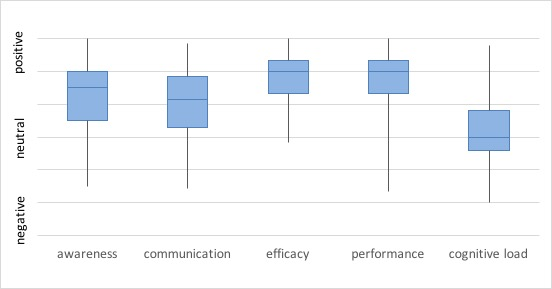
\includegraphics[width=3.00000in]{./img/survey_boxchart.jpg}
\caption{Survey responses (box shows Q1-Q3 and median; whiskers show
maximum and minimum)\label{fig:survey}}
\end{figure}

\subsection{Intertwined data modeling and data
analysis}\label{intertwined-data-modeling-and-data-analysis}

We examined the pattern of data modeling and data analysis first by
qualitatively looking at a visualization of the entire interaction log
(e.g.~Figure \autocite{fig:intertwined}a shows one team's interaction). All
teams worked intensively on data modeling as they started off the
project. This was the phase when teams were getting themselves familiar
with the documents and made initial input into CAnalytics. Starting from
certain point (e.g.~indicated by the blue dash line in the figure),
however, teams started to work on visualizations. They did not wait to
start analysis till they finished data modeling, as they returned to
making annotations again later. Indeed, the activity of data modeling
and data analysis were highly intertwined since then. Participants
switched from one activity to the other activity frequently. The state
transition diagram \autocite{fig:intertwined}b demonstrates the
interweaving in a quantitative way, in which we encode the number of
transitions as width of the link. This result confirmed our design
expectation that data modeling and data analysis should not be separate
staged activities, and that an integrated environment streamlines the
workflow.

\begin{figure*}
\centering
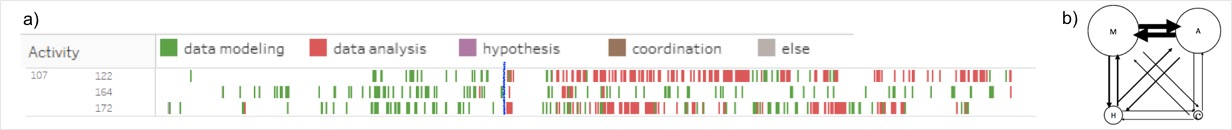
\includegraphics[width=6.5in]{./img/intertwined.jpg}
\caption{(a) Visualization of interaction logs of Team 107. Each row of
colored marks indicates the sequence of top level activities a
participant performed. (b) State transition diagram of interaction logs of Team 107. Each node is an activity, whose size represents the time spent on the it (M: data modeling; A: data analysis; H: hypothesis development; C: coordination); a
link represents a switch from one activity to another, whose width
encodes the number of switches. We see highly frequent transitions between data modeling and data analysis \label{fig:intertwined}}
\end{figure*}


\subsection{Data modeling: accretion
vs.~filtering}\label{data-modeling-accretion-vs.filtering}

\begin{figure}
\centering
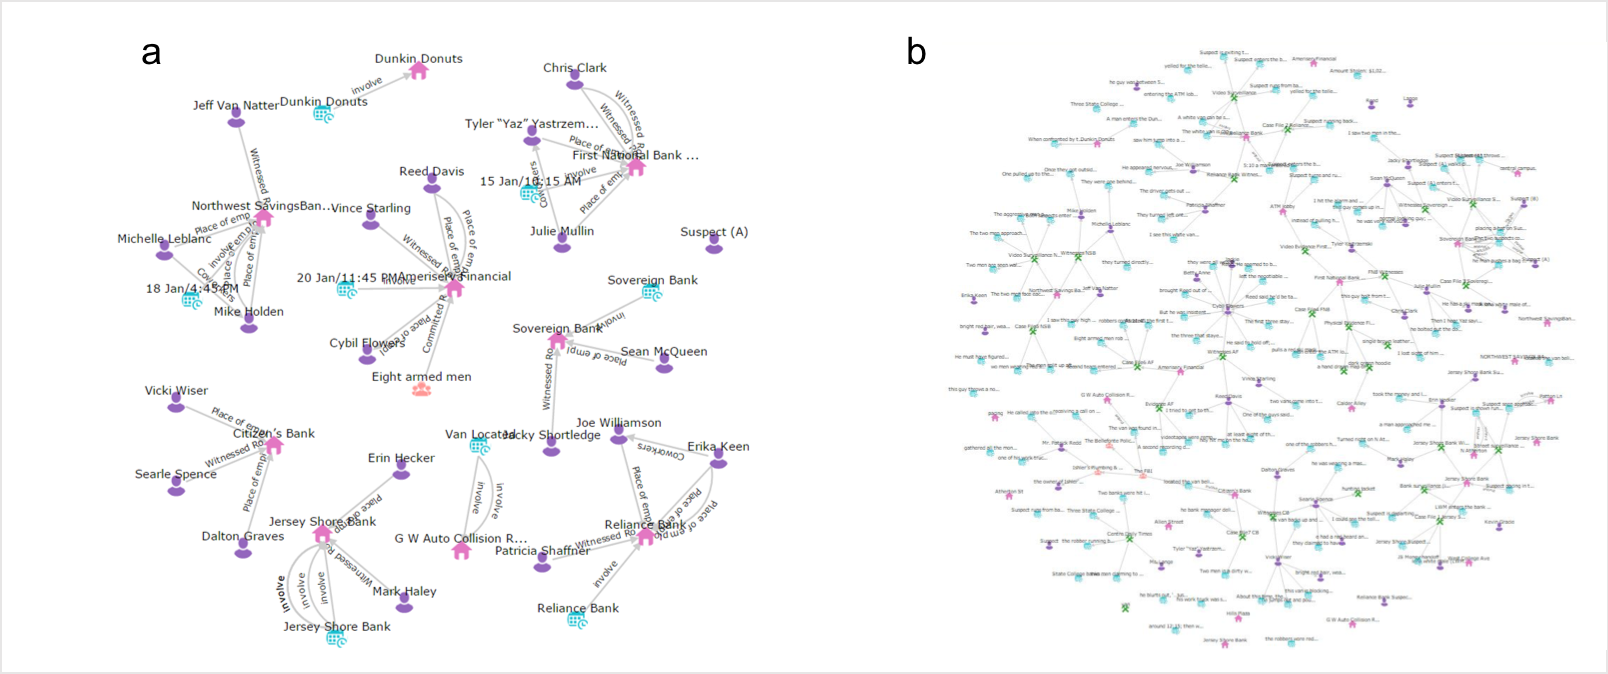
\includegraphics[width=3.20000in]{./img/network_accretion_filter.png}
\caption{Network artifact comparison: filtering (a)
vs.~accretion\label{fig:network_accretion}}
\end{figure}

From granularity of entities, We noted a distinction between accretion
and filtering strategies in data modeling, similar to what was reported in the paper prototype study. Filtering is selectively modeling of data
and adding to an artifact. Users must decide what information is
relevant, and thus what is to be excluded, as well as what granularity
of information is to model. Filtering requires more team coordination,
because teammates must reach a common ground of the current problem as
well as information needed to answer the problem. Figure
\autocite{fig:network_accretion}a is an example of filtering,
represention only the key information of robberies.

Accretion is an attempt to comprehensively represent the problem by
adding all information to an artifact. Users extract every fact from the
document, regardless of its immediate relevance to the problem.
Accretion costs less coordination as it is relatively mechanical note
taking. A disadvantage of accretion is that it could be time consuming
to model all details and the produced artifact could be fairly complex.
The strategy causes a huge variety of number of created entities and
relationships mentioned earlier. An example is Team 108, who modeled
every step the suspects took, which resulted in far more entities than
the average and more cluttered network view (Figure
\autocite{fig:network_accretion}b). Users reflected that they spent too
much time in details that they lost the bigger picture:

\begin{quote}
We would find ourselves glued to our computer screens, and spent too
much time on intelligence gathering rather than analysis (P135)
\end{quote}

While similar data modeling strategy was reported in the paper prototype
study \autocite{Carroll2013}, users with CAnalytics seemed far more
tempted to accretively add information, with far more entities and
cluttered views. Students realized in the end that many annotations did
not help them solve the problem at all because many entities were
unrelated to their problem.

\begin{quote}
I felt that after we were done annotating, we hadn't really accomplished
anything and that we were no closer to solving the case than when we had
started. In the end it didn't really help that we had annotated the
data. (P86)
\end{quote}

\subsection{Artifact construction: fact
vs.~inference}\label{artifact-construction-fact-vs.inference}

\begin{figure}
\centering
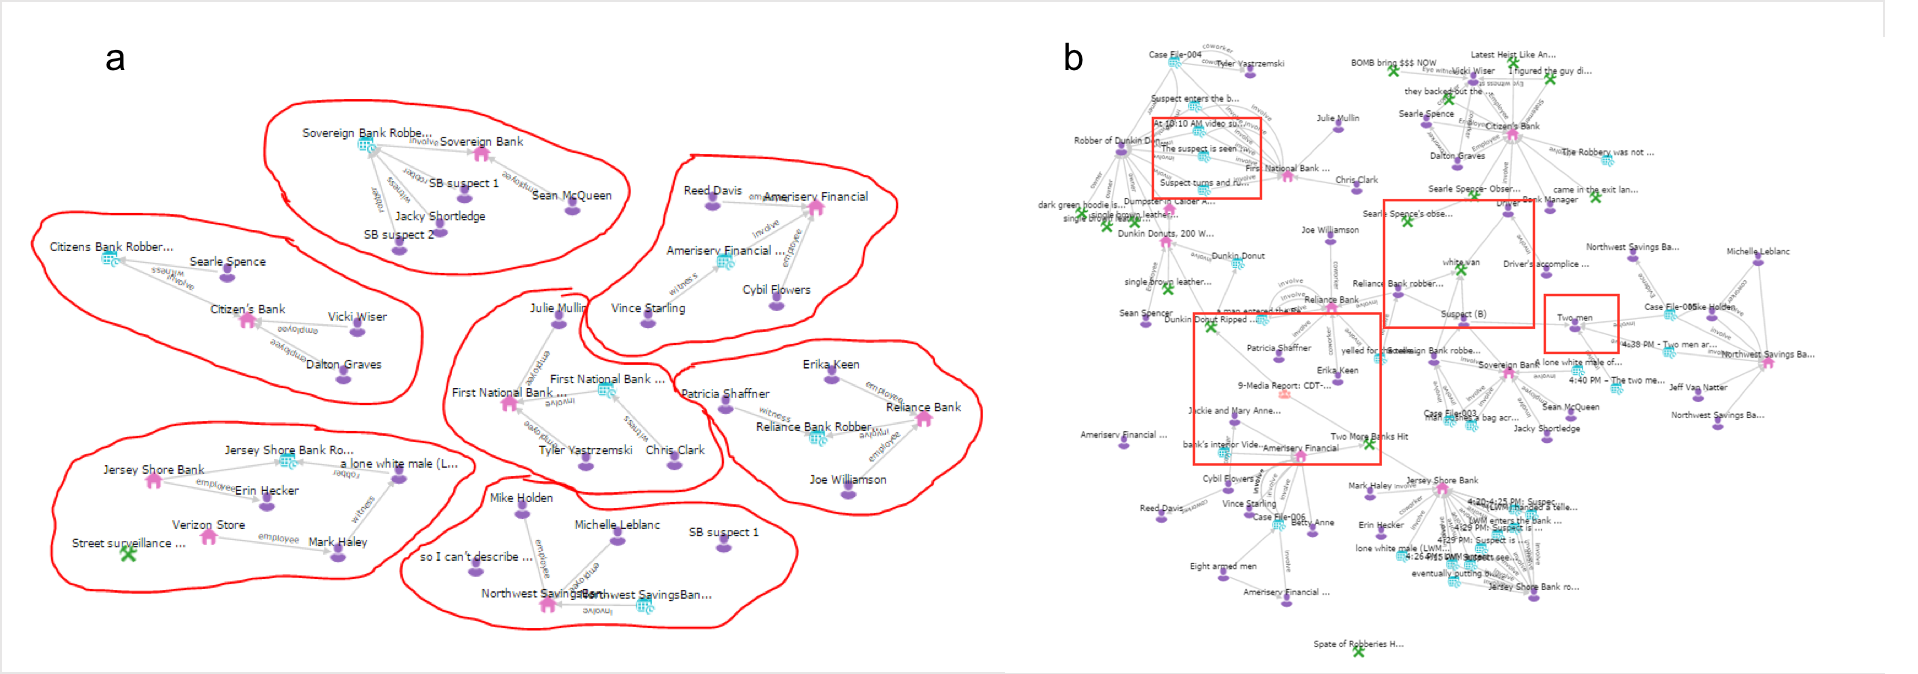
\includegraphics[width=3.20000in]{img/network_cluster.png}
\caption{Network artifact comparison: separate clusters (a)
vs.~connected clusters (b). The parts highlighted in red squares in (b) are key
evidence that connects clusters\label{fig:network_cluster}}
\end{figure}

We examined the analytic artifacts teams created, the network
graph in particular because social relationships played the most
critical role in this specific scenario and teams spent most time on
network analysis (as reflected from the log). We found the network
artifacts fell into one of two categories: the networks consisted of 1)
separate clusters, or 2) connected clusters. For example, networks from
8 teams (36\%, mean performance=7.8) consist of separate clusters
(Figure \autocite{fig:network_cluster}a). Nodes within a cluster are
connected, representing information space of a robbery case; Nodes
between clusters are nonetheless not connected, indicating each robbery
is a self-contained case. However, these teams still claimed connections
between robberies in their report. Where did they externalize these
connections? Or did the teams simply share orally and held them in mind?
It turns out that teams documented possible relationships between
robberies in the notepad tool.

In contrast, 6 other teams (mean performance=8.3) created networks
composed of connected clusters. While a cluster is still a
representation of a robbery, some of them are connected through an
evidence node. An example is Figure \autocite{fig:network_cluster}b, in
which we mark four \emph{connectors} that link the clusters. These
connectors were key evidence that led the teams to hypothesize that
those robberies were related and might be committed by the same criminal
group.

While many causes might account for the different network views, we
attempt to interpret the difference from a perspective of
\emph{uncertainty}. For instance, links within a cluster are often
factual relationships modeled from raw documents (e.g.~a white van was
witnessed at a location), but links between clusters are often
inferences beyond literally documented (e.g.~a white van at location A
is the same van witnessed at location B). Teams creating separate
clusters only represented facts in the network and held evidence with
uncertainty in a separate artifact. One advantage of distinguishing
facts and inferences is that teams can be aware of assumptions made when
making a conclusion. And since all inferences are held in one place,
teams are forced to confront them and review their uncertainty
iteratively in the process. However, the strategy also adds difficulty
to analysis as analysts may overlook or fail to combine evidence
scattered in different artifacts.

On the contrary, some other teams overlaid facts and inferences in the
same artifact. Both facts and inferences drove the layout of the
network, thus influencing team's framing of the problem. Most teams made
evaluation of the uncertainty of inferences when adding them to the
network. This strategy was relatively more interactive among teammates:
they needed to negotiate, evaluate, and reach consensus on the value and
validity of every inference. To some extent teams might forget whether a
relationship is factual or inferred, and ask whether conclusion derived
from the visualization can be trusted under uncertainty.

\subsection{Collaboration and
awareness}\label{collaboration-and-awareness}

One recurring theme in the subject feedback we collected was that the
collaboration features were helpful for solving the problem on a team
basis. In the survey 88\% of the students rated positively on their
group awareness. Participants appreciated that the tool complemented
traditional analytic tools such as Analyst's Notebook with real time
synchronization features like Google Doc, and added visual analytics to
Google Doc which only supports text writing. To quote one participant,
\emph{``CAnalytics is like an analysts notebook that multiple people
could work on at once {[}\ldots{}and{]} an analysts version of a Google
Doc.''} (P65). For example, participants reflected that they could now
contribute simultaneously without concerns of interference and could
have everything in one place instead of manually sharing documents using
cloud service.

\begin{quote}
It was much easier to coordinate as a team with CAnalytics because we
could all work on the same system at the same time. Without CAnalytics,
we were forced to do the work separately and compile all the work onto
one system after we had finished. (P156)
\end{quote}

Students also reported that being able to see teammate's status made the
task more motivating and engaging:

\begin{quote}
During class I wasn't sure if my teammates were doing work for that
class or another thing but then seeing their dot {[}tool indicator{]}
switch between applications on the software and updates pop up on my
screen I knew they were doing work for 231. (P141)
\end{quote}

\begin{quote}
The fact that you can see what other teammates are doing and they can
see what you are doing creates a sense of accountability in terms of
separating the work load. (P51)
\end{quote}

Another repeated theme was awareness that all teammates were executing
the team plan. Participants reflected on their experience that a common
team breakdown was misunderstanding of the team plan. Teammates thought
they had reached agreement to a plan till in the end to find no
collaborators were doing the things as expected. CAnalytics made it
easier because they could always see if teammates were doing the
expected work; and if not, they could communicate immediately rather
than in the end of the project.

Participants reported many other instances of awareness they realized
using CAnalytics. We categorized them based on the element of awareness,
or the essential problem of awareness of \emph{what}
\autocite{Schmidt2002}, into social awareness, information awareness,
action awareness, history awareness, and intention awareness, as shown
in Table \autocite{tab:awareness}.

When asked what features helped them stay aware of team activities, 28
participants mentioned the tool coordinator, 24 mentioned the
notification system, 19 mentioned the history tool, 14 mentioned the
real-time update of user-generated data, 12 mentioned the collaborative
editor, and 7 mentioned the message tool. While the number of mentions
does not simply indicate tool usefulness, it suggests users appropriate
these features and were explicitly aware of their support.

% Please add the following required packages to your document preamble:
% \usepackage[table,xcdraw]{xcolor}
% If you use beamer only pass "xcolor=table" option, i.e. \documentclass[xcolor=table]{beamer}
% \usepackage[normalem]{ulem}
% \useunder{\uline}{\ul}{}
\begin{table*}[]
\centering
\small
\label{tab:awareness}
\begin{tabular}{p{3cm}p{10cm}}
\rowcolor[HTML]{9B9B9B}
\multicolumn{1}{c}{\cellcolor[HTML]{9B9B9B}\textbf{Element}}                           & \multicolumn{1}{c}{\cellcolor[HTML]{9B9B9B}\textbf{Example}}                                                                                                                                                                                                                                                                                                                                 \\
\rowcolor[HTML]{C0C0C0}
\begin{tabular}[c]{@{}l@{}} Social awareness\\ \emph{who is present?}\end{tabular}             & CAnalytics helped me stay aware,of my teammates activities because I could see who was logged on in the top,right corner (P123)                                                                                                                                                                                                                                                              \\
\rowcolor[HTML]{EFEFEF}
\begin{tabular}[c]{@{}l@{}}History awareness\\ \emph{Who has done what?}\end{tabular}         & The way you are able to view when and where your teammate made or updated annotations/information was the key to staying aware of what your team has done. It is a great tool in respects to that. For example, I was able to view the changes my team made while I was not using the CAnalytics tool at the same time they were using the history tab. (P171)                               \\
\rowcolor[HTML]{9B9B9B}
\begin{tabular}[c]{@{}l@{}}Information awareness\\ \emph{What is being changed?}\end{tabular} & CAnalyitics was very helpful in keeping us updated on what was being changed/noted/amended by whom and when. This was very beneficial for staying on the same page and knowing what changes were being made so no one individual was out of the loop. (P157)                                                                                                                                 \\
\rowcolor[HTML]{EFEFEF}
\begin{tabular}[c]{@{}l@{}}Action awareness\\ \emph{Who is doing what?}\end{tabular}          & I liked how you could always see what your teammate were viewing on the website. For example I was working on the bluf when my teammates were working on the network part of the program. If I were to come across a piece of information that I thought might be helpful to them I would just tell them. My teammates did the same thing in return. (P51)                                   \\
\rowcolor[HTML]{C0C0C0}
\begin{tabular}[c]{@{}l@{}}Intention awareness\\ \emph{Who is going to do what?}\end{tabular} & CAnalytics showed what tab {[}tool{]} my teammates were working on which helped me be aware of what they were working on. For example, if I saw that one of my teammates was on the network tab, I knew that they were attempting to connect the information that was relevant to one another.,I would then be able to mention any new findings I had that could influence their work (P160)
\end{tabular}
\caption{Subject feedback of awareness instances}
\end{table*}


Students' positive feedback on awareness was further corroborated by
interaction logs. For example, we measured the number of entities
accessed by collaborators versus by the author only. While data
generated by users is automatically shared, it is up to collaborators to
choose to read the shared information or ignore information altogether.
A high awareness team would keep updated with collaborators' generated
information and read information soon after it is shared; whereas a low
awareness team might experience a significant delay or even never access
it. We found that most teams shared a high proportion of entities
(M=77.6\%). We found that in average, 77.6\% of the created entities
were accessed by at least one teammate.

One major critique is the lack of sharing of intermediate analytic
insights in close collaboration. To gain insights individuals are
constantly exploring and rearranging visualizations. For example,
analysts can apply a filter to have a reduced data view of interest,
highlight an area to sharpen analytic focus, and re-layout the node-link
graph to make their own cluster of relevant entities. While the shared
data pool represents the information the team have in common, views of
data reflect and contextualize individual's \emph{interpretations}
toward the data. The view together with its interpretation represents
user's intermediate analytic status. While it may not be a mature
hypothesis or conclusion, the intermediate insight is still worth
sharing because it may inspire collaborators. With CAnalytics
participants complaint that they could not easily communicate insight
together with the associate views to the team. The team could \emph{``be
looking at the same information but arranged in completely different
ways'' (P131)}.

\subsection{Collaboration strategies}\label{collaboration-strategies}

We noted different collaboration strategies from interaction logs. Seven
teams followed \emph{document-based collaboration}: they divided their
work by evenly distributing the provided documents among team members
(as shown in Figure \autocite{fig:labor_division}a). Each member read
through and made annotations on their own set of documents. An advantage
of this strategy is that individuals get less workload and thus have
more time to think deep into their own documents. Individuals also
implicitly take over the responsibility of their assigned documents to
gain insights and share them when the team synthesize findings in later
analysis. When the team needs information from one document, they rely
on the ``document owner'' to share his/her finding. The fallback of this
strategy is thus in case an individual fails to identify or convey
evidence in the document, the team may overlook the information
altogether \autocite{Borge2012}.

In contrast, four teams followed an \emph{entity-based collaboration}
strategy. Instead of dividing by documents, they divided work by entity
types: each individual went through all documents but only annotated
entities of certain types, e.g.~teammate A only annotated persons and
teammate B annotated locations (as shown in Figure
\autocite{fig:labor_division}b). This strategy saves teammate's time on
data modeling. And since each person focuses only on certain entities,
they are more likely to identify recurring patterns, for example, the
white van used in multiple robberies. However, focusing on certain
entities could lead individuals to superficial syntactic scanning of
documents instead of deep reading. This could further lead to extremes
of annotating all entities of the type, whether they are related to the
problem at hand or not. We found from the interaction log that EBC teams
created more entities (M=101) in average than DBC teams (M=94.5), which
seems to back our guess. Moreover, with emphasis on certain entities,
individuals are likely to know only partial aspects of a robbery and
hence have difficulty connecting and synthesizing facts to deduce any
conclusion. As one participant reflected, \emph{``we broke up by entity
type, which reduced our individual involvement in each other's entity
types (P99).''} The average performance of EBC teams (M=7.63) was lower
than that of DBC teams (M=9.25), which seems to confirm our analysis,
although the difference was not statistically significant.

The rest (eleven) of the teams did not show specific labor division
patterns. Indeed, teams did not necessarily have to divide their work in
order to collaborate, especially when the collaborative tool provides
possibility to work closely together. Teammates could read and annotate
the same document because they could see new annotations by others in
real time and build on other's annotation. Figure
\autocite{fig:close_collaboration} shows an example where one team
worked on the same document simultaneously. This has the advantage that
teammates are always on the same page and can discuss hypotheses
throughout the analysis process. Participants did have concern for
possible duplication. As one participant complaint, ``we could not
actively see the changes our teammates were making until well after they
had made them.(P46)'' This was because an annotation was shared only
\emph{after} it was created, yet another teammate might be drafting an
annotation in the meantime.

\begin{figure}
\centering
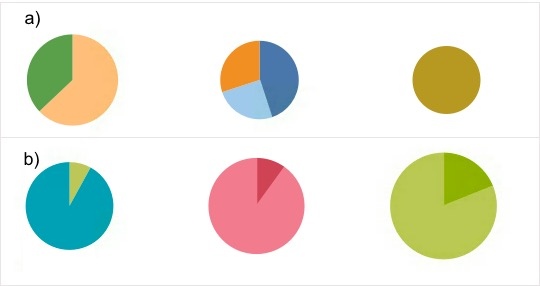
\includegraphics[width=3.20000in]{img/labor_division.jpg}
\caption{Pie charts showing different labor division strategies. Each
pie chart corresponds to one team member. (a) Document-based
collaboration. The pie chart shows the documents one team member
annotated, color coded by document ID. (b) Entity-based collaboration.
The pie chart shows the entity types one team member created, color
coded by entity types.\label{fig:labor_division}}
\end{figure}

\begin{figure}
\centering
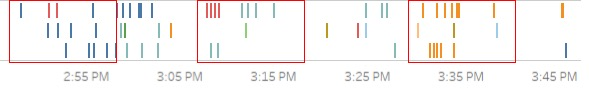
\includegraphics[width=3.20000in]{img/close_collaboration.jpg}
\caption{Graph showing the timeline of one team creating annotations.
Each row corresponds to one team member. Each bar represents an
annotation, color coded by document ID. The red blocks highlights the
periods when all teammates worked on the same documents
simultaneously.\label{fig:close_collaboration}}
\end{figure}
